%%%%%%%%%%%%%%%%%%%%%%%%%%%%%%  IEEEsample.tex
%%%%%%%%%%%%%%%%%%%%%%%%%%%%%%%%%%%%%%%%%
%%%%%%%%%%%%%%%%%%%%%%%    More information: see the header of IEEEtran.sty
%%%%%%%%%%%%%%%%%%%%%%%
%%%%%%%%%%%%%%%%%%%%%%%%%%%%%%%%%%%%%%%%%%%%%%%%%%%%%%%%%%%%%%%%%%%%%%%%%%%%%%%%
%%%%

\documentclass[conference,10pt]{IEEEtran}
%\documentclass[conference]{IEEEtran}

%%%\IEEEoverridecommandlockouts

\usepackage[ruled]{./algorithm2e}
%%for algorithm2e package, label has to be following caption in the same line!!!
\renewcommand{\algorithmcfname}{ALGORITHM}
\SetAlFnt{\small}
\SetAlCapFnt{\small}
\SetAlCapNameFnt{\small}
\SetAlCapHSkip{0pt}
\IncMargin{-\parindent}



%% \RequirePackage{times}
%% \RequirePackage{algorithmic}
%% \PassOptionsToPackage{boxed}{algorithm}
%% \RequirePackage{algorithm}
%% \RequirePackage{multicol}
%\renewcommand{\algorithmicrequire}{\textbf{Inputs:}}
%\renewcommand{\algorithmicensure}{\textbf{Outputs:}}
%\DeclareMathAlphabet{\mathtsl}{OT1}{ptm}{m}{sl}

%\def\BibTeX{{\rm B\kern-.05em{\sc i\kern-.025em b}\kern-.08em1
%    T\kern-.1667em\lower.7ex\hbox{E}\kern-.125emX}}

%\newtheorem{theorem}{Theorem}
%\newtheorem{lemma}{Lemma}
%\newtheorem{example}{Example}
%\newtheorem{corollary}{Corollary}

\RequirePackage{amssymb, mathptm}
\usepackage{amsbsy}
\usepackage{graphicx}
\usepackage{helvet}
\usepackage{enumerate}
\usepackage{amsmath}
\usepackage{amsfonts}
\usepackage{graphicx}
\usepackage{multirow}
\usepackage{subfig}
\usepackage{comment}
\usepackage{leqno}
\usepackage{cases}



%%indent in algorithm


%\setcounter{page}{1}


% New command for the table notes.
\def\tabnote#1{{\small{#1}}}

% New command for the line spacing.
\newcommand{\ls}[1]
    {\dimen0=\fontdimen6\the\font
     \lineskip=#1\dimen0
     \advance\lineskip.5\fontdimen5\the\font
     \advance\lineskip-\dimen0
     \lineskiplimit=.9\lineskip
     \baselineskip=\lineskip
     \advance\baselineskip\dimen0
     \normallineskip\lineskip
     \normallineskiplimit\lineskiplimit
     \normalbaselineskip\baselineskip
     \ignorespaces
    }
%\renewcommand{\algorithmicrequire}{\textbf{Input:}}
%\renewcommand{\algorithmicensure}{\textbf{Output:}}

\newcommand{\beq}{\begin{equation}}
\newcommand{\eeq}{\end{equation}}
\newcommand{\beqarr}{\begin{eqnarray}}
\newcommand{\eeqarr}{\end{eqnarray}}
%\newcommand{\ov}{\overline}
\newcommand{\ov}{\bar}
\newcommand{\xor}{\bigoplus}
\newcommand{\Fm}{{\mathbb{F}}}



%the following is for space before and after align or other equation environment.

%%
\newtheorem{Algorithm}{Algorithm}[section]
\newtheorem{Definition}{Definition}[section]
\newtheorem{Example}{Example}[section]
\newtheorem{Proposition}{Proposition}[section]
\newtheorem{Lemma}{Lemma}[section]
\newtheorem{Theorem}{Theorem}[section]
\newtheorem{Corollary}{Corollary}[section]
\newtheorem{Conjecture}{Conjecture}[section]
\newtheorem{Problem}{Problem}[section]
\newtheorem{Notation}{Notation}[section]
\newtheorem{Setup}{Problem Setup}[section]
%%%

%%set spacing between table columns
\setlength{\tabcolsep}{3pt}

\begin{document}

%\thispagestyle{empty}
%\pagestyle{empty}

\title{Class Project Report: Boundary-free Technology Mapping using Gr\"obner Basis}

\author{
\IEEEauthorblockN{Xiaojun Sun}
\IEEEauthorblockA{Electrical and Computer Engineering\\
University of Utah\\
Salt Lake City, Utah 84112\\
Email: xiaojuns@ece.utah.edu}
}

%%\author{\IEEEauthorblockN{Jinpeng Lv and Priyank Kalla}\thanks{This work is sponsored in part by a grant from NSF \#CCF-546859.}
%\IEEEauthorblockA{Department of  Electrical and Computer Eng.\\
% University of Utah, Salt Lake City, UT-84112 \vspace{-0.3in}
 %\{lv, kalla\}@eng.utah.edu
% }
%\and
%\IEEEauthorblockN{Florian Enescu} \thanks{\normalsize  978-3-9810801-8-6/DATE12/$\copyright 2012$ EDAA}
%\IEEEauthorblockA{Department of Mathematics and Statistics\\
% Georgia State University,  Atlanta, GA 30302-4038 \vspace{-0.3in}
% fenescu@mathstat.gsu.edu
%} 
%
 
\maketitle

%\markboth{MS Proposal by Tim Pruss}{}
\newcommand{\Fq}{{\mathbb{F}}_{q}}
\newcommand{\Fkk}{{\mathbb{F}}_{2^k}}
\newcommand{\Fkkx}[1][x]{\ensuremath{\mathbb{F}}_{2^k}[#1]\xspace}
\newcommand{\Grobner}{Gr\"{o}bner\xspace}
\newcommand{\B}{{\mathbb{B}}}
\newcommand{\Z}{{\mathbb{Z}}}
\newcommand{\F}{{\mathcal{F}}}
\newcommand{\G}{{\mathcal{G}}}
\newcommand{\R}{\mathbb{R}}
%%%

\newcommand{\debug}[1]{\textcolor{gray}{[ #1 ]}}


%\thispagestyle{empty}

%%%%%%%%%%%%%%%%%%%% Include your files here %%%%%%%%%%%%%%%%%%%%%
\begin{abstract}
As FPGA is widely used in hardware implementation and the size of design is usually large, there 
is an increasing need in industrial domain for an approach that can map macro blocks. Currently
there is no algorithms can map large-scale functions without boundary information, especially
arithmetic blocks in datapath. Our approach provides an alternative inspiration to solve
this problem using Gr\"obner basis based ideal membership test, whose efficiency does not
rely on the complexity of arithmetic block's inner structure.
\end{abstract}

\section{Introduction}
\subsection{Problem Description}
One sentence on this problem is: find a method to map the macro blocks without boundary information.
Mapping is an essential technique used in synthesis and verification. In synthesis, we can map the 
macro functions with smaller and faster implementations to optimize the timing and area; in simulation,
we can map a complicated function to a simple execution to accelerate simulation speed.

Given a gate-level design $D$ and several word-level macro blocks $\{B_i\}$, we need to map macro
blocks $B_i$ into design $D$, and write out the mapped design $D'$ which is equivalent to original
design $D$. The objective is to generate a mapped design $D$ with as many of $B_i$ such that the area
and timing is optimal. 

\begin{figure}[hbt]
	\begin{center}
	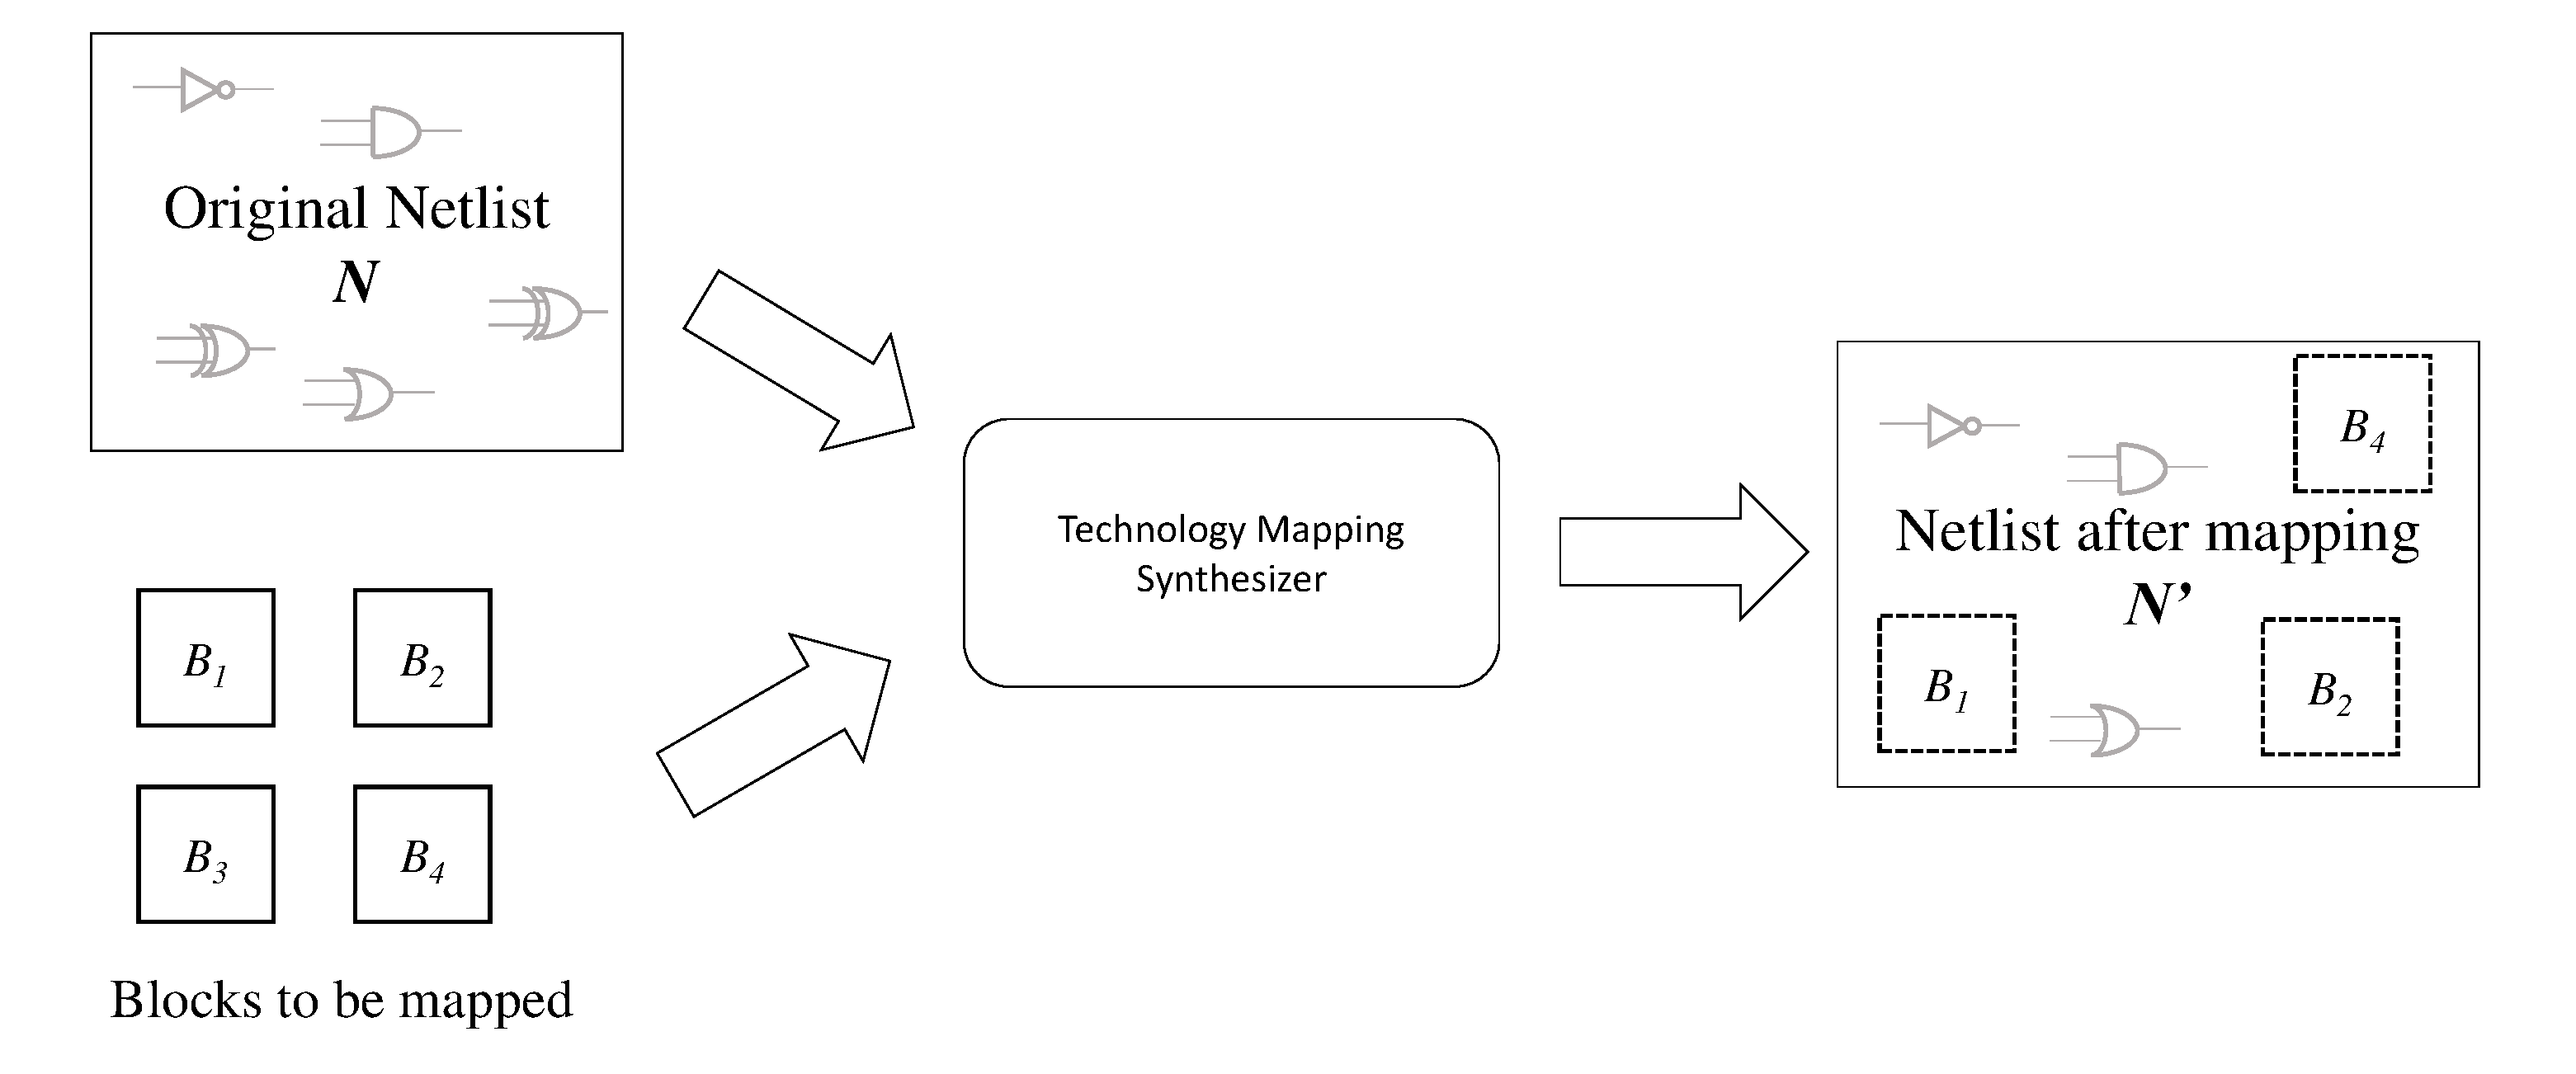
\includegraphics[scale=0.3]{macro.png}
	\end{center}
	\caption{The outline and flow of mapping for macro blocks}
	\label{fig:macro}
\end{figure}

\section{Preliminaries}
\label{sec:intro}

\subsection{Modeling of constrains by ideal}
A state can be described by a set of constrains. Generally speaking, a constrain is a function mapping 
from variables to boolean values ($f:X\to bool,\ X=\{x_0,\dots,x_n\}$); meanwhile this "function" can be
written in form of polynomial about variables. If the constrain is satisfied, i.e. $f:\sigma(X)\to \perp$,
accordingly the evaluation of this polynomial is 0:
$$f(x_0,\dots,x_n) = a_0x_0+\cdots + a_nx_n = 0$$
If a state is valid under some interpretation, then all of its constrains need to be satisfied:
\begin{equation}
\left\{
\begin{array}{ll}
f_0(x_0\dots x_n) = 0\\
\vdots\\
f_k(x_0\dots x_n) = 0
\end{array}\right.
\nonumber
\end{equation}
It is reasonable to consider the solution vector $\langle x_0,\dots,x_n\rangle$ for this system of 
equations. However in most cases, solving the system is impossible and unnecessary; instead people
tend to generate a simpler constrain/polynomial as an over-approximation (also known as \emph{abstraction})
from heuristic methods and then check if it satisfies all constrains of this state, which means
$$\forall j, f_j(\langle x_i\rangle) = 0\implies\F(\langle x_i\rangle) = 0  $$
One heuristic is to take $\F$ as composition of $\langle f_j\rangle$ as follows: if
$$\F = c_0f_0+c_1f_1+\cdots+c_kf_k$$
then above implication can hold. Here coefficients $c_j$ could be any polynomials
or real numbers. Now review Definition 2 in original paper:
\begin{Definition}
{\bf Ideals:}\ \ An \emph{ideal} $J$ generated by polynomials $f_0,\dots,f_k\in \mathbb{F}_q[x_0,\dots,x_n]$
is defined as $$J = \langle f_0,\dots,f_k\rangle = \{\sum_{i=0}^{k}c_i\cdot f_i\ |\ c_i\in\mathbb{F}_q[x_0,
\dots,x_n]\}$$
$f_0,\dots,f_k$ are called \emph{generators} of ideal $J$.
\end{Definition}
Thus we can formally say
\begin{Theorem}
If $f_0\sim f_k$ are all satisfied and $\F$ belongs to the \emph{ideal} generated by $\{f_0,\dots,f_k\}$, then
$\F$ is also satisfied.
\end{Theorem}

\subsection{Ideal membership and Gr\"obner basis}
From last section, to check if $\F$ is a valid abstraction, it is necessary to check if 
$\F\in J=\langle x_0,\dots,x_n\rangle$, this requires a technique called \emph{ideal membership test}.
To execute this technique, $\langle f_0,\dots,f_k\rangle$ need to be transformed to \emph{Gr\"obner Basis}
$\langle g_0,\dots,g_s\rangle$.

Gr\"obner basis can generate the same ideal as from original generators. Meanwhile it has an important property
that the leading term from an arbitrary polynomial from this ideal can be divided by at least one Gr\"obner
basis polynomial's leading term. More specifically,
\begin{Definition}
{\bf Gr\"obner Basis:}\ \ For a monomial ordering $>$, a set of non-zero polynomials $G=\{g_0,\dots,g_s\}$
contained in an ideal $J$, is called a \emph{Gr\"obner basis} for $J$ if and only if:
$$\forall f\in J, f\neq 0, \exists g_i\in G: lm(g_i)\ |\ lm(f)$$
where $lm$ denotes the leading monomial of a polynomial.
\end{Definition}

This property is vital when operating following "multi-division":
\begin{Definition}
{\bf Multi-division:}\ \ A polynomial $f$ divided by an ideal $J$(actually its generators, a finite set of
polynomials) follows rules from multi-division $f\xrightarrow{J}$:\\
for each term $t$ in $f$, search in all generators of $J$ such that the leading monomial of $g_i$ can divide
this term's monomial, then update $f$:
$$f = f - \frac{t}{lt(g_i)}g_i$$
$lt$ means leading term. Every time $\frac{t}{lt(g_i)}$ is recorded as one term of quotient $c_i$ w.r.t. $g_i$.
When it is impossible to update $f$, the value of $f$ is recorded as \emph{remainder} $r$, denoted as
$f\xrightarrow{J}_{+}r$.
\end{Definition}

If $J = \langle f_0,\dots,f_k\rangle$, $\F\xrightarrow{J}_+r$, apparently we have
$$\F = c_0f_0+c_1f_1+\cdots+c_kf_k + r$$
if the remainder $r=0$, then $\F$ is the desired constrain ($\F\in J$). Now look back to the property of
Gr\"obner basis, when $\F\in J$, then every step updated $\F$ also belongs to $J$, which means for every
term in original $\F$ we can find corresponding $g_i$ whose leading term can divide it, thus the remainder
will be 0. Reversely if remainder is 0, we can also deduce $\F\in J$.

\begin{Theorem}
{\bf Ideal membership:}\ \ For ideal $J=\langle g_0,\dots,g_s\rangle$ and $\{ g_0,\dots,g_S\}$
is a Gr\"obner basis, polynomial $\F\in J$ if and only if $\F\xrightarrow{J}_+0$.
\end{Theorem}
\subsection{Buchberger's Algorithm}
\label{sec:buch}
Buchberger's algorithm
shown in Algorithm \ref{alg:gb},  computes a Gr\"obner
basis over a field. Given polynomials $F = \{f_1, \dots, f_s\}$, 
the algorithm computes the Gr\"obner basis $G = \{g_1, \dots, 
g_t\}$.
% such that ideal $I = \langle f_1, \dots, f_s\rangle = \langle g_1,
% \dots, g_t\rangle$. 
In the algorithm,  

\begin{equation}
       Spoly(f,g)=\frac{L}{lt(f)}\cdot f - \frac{L}{lt(g)}\cdot g \nonumber
      \label{eqn:spoly}
\end{equation}
where $L = \text{LCM}(lm(f), lm(g))$, where $lm(f)$ is the leading
monomial of $f$, and $lt(f)$ is the leading term of $f$. 


\begin{algorithm}[hbt]
\SetAlgoNoLine
 \KwIn{$F = \{f_1, \dots, f_s\}$}
 \KwOut{$G = \{g_1,\dots ,g_t\}$\\} %, a Gr\"{o}bner basis
  $G:= F$\;
  \Repeat{$G = G'$}
  {
  	$G' := G$\;
  	\For{ each pair $\{f, g\}, f \neq g$ in $G'$} 
	{
		$Spoly(f, g) \stackrel{G'}{\textstyle\longrightarrow}_+r$ \;
		\If{$r \neq 0$}
		{
			$G:= G \cup \{r\}$ \;
		}
	}
   }
\caption {Buchberger's Algorithm}\label{alg:gb}
\end{algorithm}

\subsection{Elimination using Gr\"obner Basis}
\label{sec:elim}
We are given a circuit $C$ with $k$-bit inputs and outputs that
performs a polynomial computation $Y = \F(A)$ over $\Fq = \Fkk$. Let
$P(x)$ be the {\it given} irreducible or primitive polynomial used for
field construction, and let $\alpha$ be its root, i.e. $P(\alpha) = 0
$. Note that we do not know the polynomial representation
$\F(A)$ and our objective is to identify (the coefficients of)
$\F(A)$. Let $\{a_0, \dots, a_{k-1}\}$ denote the primary inputs and
let $\{y_0, \dots, y_{k-1}\}$ be the primary outputs of $C$. Then, the
word-level and bit-level correspondences are: 
\begin{equation}
\label{eqn:words}
 A = a_0 + a_1 \alpha + \dots + a_{k-1} \alpha^{k-1}; ~~ Y = y_0 +
y_1 \alpha + \dots + y_{k-1} \alpha^{k-1};
\end{equation}

We analyze the circuit and model all the gate-level Boolean operators
as polynomials in ${\mathbb{F}}_2 \subset \Fkk$. To this set of
Boolean polynomials, we append the polynomials of Eqn
(\ref{eqn:words}) that relate the word-level and bit-level
variables. We model this set of polynomials as $F = \{f_1, \dots,
f_s\}$ over the ring $R = \Fq[x_1, \dots, x_d, Y, A]$. Here $x_1,
\dots, x_d$ denote, collectively, all the bit-level variables of the
circuit --- i.e. primary inputs, primary outputs and the intermediate
circuit variables --- and $Y, A$ the word-level variables. Denote the
generated ideal as $J = \langle F \rangle \subset R$. As $Y = \F(A)$
is a polynomial representation of the circuit, represent this (unknown)
``specification'' as a polynomial $f: Y - \F(A)$, or as $f: Y + \F(A)$
and $-1 = +1$ over $\Fkk$.  

As the circuit $C$ implements the function $f$, clearly $f$ {\it
  agrees with the solutions} to $f_1 = \dots = f_s = 0$. In computer
algebra terminology, this means that $f$ {\it vanishes on the variety} 
$V_{\Fq}(J)$. If $f$ vanishes on $V_{\Fq}(J)$, then $f$ is a member of
the ideal $I(V_{\Fq}(J))$. Strong Nullstellensatz over Galois fields tells us that $I(V_{\Fq}(J)) =
J + J_0$, where $J_0 = \langle x_1^q - x_1, \dots, x_d^q - x_d, Y^q -
Y, A^q - A \rangle$ is the ideal of vanishing polynomials in
$R$. Consolidating these results, we deduce that the specification
polynomial $f \in (J+J_0)$. 

If the specification polynomial is known, then the verification
problem can be solved using membership testing of $f$ in the ideal $(J
+ J_0)$. We will now show
that by computing a Gr\"obner basis of $(J + J_0)$, using a specific
elimination term order, we can also identify the polynomial $f$ which
represents the function implemented by the circuit.

Moreover, Gr\"obner bases may be used to generate an elimination ideal
by using an ``elimination order.''  One such ordering
is a pure lexicographic ordering, which features into a theorem:
%The ideal $I_k$ is spanned by elements which eliminate variables
%$x_1,\dots,x_k$.  This leads to an {\bf elimination theorem} for \Grobner
%bases:
\begin{Theorem} \label{thm:elim}
({\bf Elimination Theorem}) Let $J
  \subset \Fq[x_1,\dots,x_d]$ be an     ideal and let $G$ be a
  Gr\"obner basis of $J$ with respect to a lex ordering where $x_1
  > x_2 > \dots > x_d$.  Then for every $0     \leq l \leq
  d$, the set 
    \begin{equation}
        G_l= G \cap \Fq[x_{l+1},\dots,x_d]
    \end{equation}
    is a Gr\"obner basis of the $l$th elimination ideal $J_l$.
\end{Theorem}

Gr\"obner basis computations w.r.t. pure lexicographic
term orders can be used to eliminate variables from an ideal. The
above example motivates our approach: Since we want to derive a
polynomial representation from a circuit in variables $Y, A$, we can
compute a Gr\"obner basis of $J + J_0$ w.r.t. an elimination order
that eliminates all the ($d$) bit-level variables of the
circuit. Then, the Gr\"obner basis $G_d = G \cap \Fq[x_1, \dots, x_d,
  Y, A]$ of the $d^{th}$ elimination ideal of $(J + J_0)$ will contain
polynomials in only $Y, A$. We now prove that the 
required polynomial representation will be found in $G_d$.

\section{Techniques from Loop Invariant paper}
This section briefly illustrates S. Sankaranarayanan's POPL'04 conference paper.
First, a transition system is modeled by algebraic assertions; then \emph{ideal membership test}
is applied on the set of assertions to help abstract the loop invariant. "Template" is the concept
I borrowed from this paper to apply on my own approach.
\subsection{Template and state constrains}
\label{sec:basic}
To effectively and efficiently utilize the ideal membership test technique, a heuristic to
generate $\F$ is needed. One heuristic can provide better coverage for loop invariant abstraction as well as
relatively small size is \emph{generic quadratic form}.

For example, a pair of state variables $\{x,y\}$'s generic quadratic form is
$$\F = a_0x^2+a_1x+a_2xy+a_3y+a_4y^2+a_5$$
It covers all possible terms with degree at most 2. $a_0\sim a_5$ are usually real number parameters,
a certain assignment about them can turn $\F$ into desired invariant. This parameterized constrain
polynomial covers all combinations of state variables can also be called a \emph{template}.

Finding a proper assignment is the major part of original paper and has potential to be even further explored
beyond that paper, and/or to be applied on different research field.
\subsection{Modeling initial state}
\label{sec:CKR}
For initial state, the constrains are explicit. A template is adopted and refined by Gr\"obner basis 
generated by original constrains, by equaling the remainder to 0 we can get constrains on
parameters from the template.

An example is Fig.\ref{fig:loopinv}. The template is generic quadratic form of $\{s,i,j,j_0\}$, which is
\begin{figure}[hbt]
	\begin{center}
	\includegraphics[scale=0.3]{../../../Pictures/Selection_006.png}
	\end{center}
	\caption{An example program of 2 Natural numbers' multiplication (Fig.1 from original paper)}
	\label{fig:loopinv}
\end{figure}
\begin{align}
\F =& a_0s^2+a_1s+a_2si+a_3sj+a_4sj_0\nonumber\\
&a_5i^2+a_6i+a_7ij+a_8ij_0+a_9j^2\nonumber\\
&a_{10}j+a_{11}jj_0+a_{12}j_0^2+a_{13}j_0+a_{14}\nonumber
\end{align}

Constrains of initial state: $s=0\land j=j_0$ can be interpreted to polynomials:
$\{s, j-j_0\}$. Check if it is Gr\"obner basis using \emph{Buchberger's algorithm}. Since
their leading terms are relatively prime, we can write Gr\"obner basis $G=\{s, j-j_0\}$. Its ideal
$J=\langle s,j-j_0\rangle$.

Compute multi-division $\F \xrightarrow{G}_+ r$, the remainder is
$r = a_5i^2+a_6i+(a_7+a_8)ij_0+(a_9+a_{11}+a_{12})j_0^2+(a_{10}+a_{13})j_0+a_{14}$.
Let it equal to 0, each coefficient will generate a constrain, solution to the system is candidate
assignment to generate invariant.
\begin{equation}
\left\{
\begin{array}{l}
a_5=a_6=a_{14}=0\\
a_7+a_8=0\\
a_9+a_{11}+a_{12}=0\\
a_{10}+a_{13}=0
\end{array}\right.
\nonumber
\end{equation}

\subsection{Modeling state transitions}
2 states get involved in a state transition. The technique requires to model the 2 states individually,
do multi-division separately to get remainder $r_1$ and $r_2$. Suppose a constrain polynomial for
this transition is $r_t$, we requires that when invariant for state 1 holds and transition $1\to 2$ stands,
invariant for state 2 should also holds, which is
$$(r_1 = 0)\land (r_t = 0) \implies (r_2 = 0)$$
One reasonable conjecture is
$$r_t = r_1 - \lambda r_2$$
Theoretically $\lambda$ could be any polynomial. Consider the system to be easy to solve, we keep $\lambda$
only taking value from real numbers.

Still take Fig.\ref{fig:loopinv} as example (also refer to Example 10 in original paper). State 1 is initial state we 
just characterized $\F = f(s,i,j,j_0)$, and the post state (state 2) have exactly the same form constrain:
$\F' = f(s',i',j',j_0')$. Considering transition relation, substitute $s'$ with $s+i$, replace $j'$
with $j-1$, and $i'$ for $i$, $j_0'$ for $j_0$, the template for state 2 is expression $f'$ in Example 10 from
original paper.

Do multi-division with Gr\"obner basis generated by transition relation, record its remainder $r_2$.
From equality $r_2 = \lambda r_1$, we get constrains for parameters. Solve the system using covering-problem-like
techniques (Part. \emph{Elimination by Splitting} in original paper). One branching result is:
$a_0,a_2\sim a_6, a_9\sim a_{14}$ are all zero; $a_1=a_7=-a_8$. Then reduced remainder 
$$r_2 = a_1s +(a_1-a_7)i+a_7ij+a_8ij_0 = a_1(s+ij-ij_0) = 0$$
Desired invariant is 
$$s = i(j_0- j)$$
We knew the program calculates $i\times j_0$. Initially $s=0$, $j_0-j=0$, invariant holds;
during each cycle, $s'=s+i, (j_0'-j') = (j_0-j)+1$, the invariant also holds. In conclusion, this is a
loop invariant for program in Fig.\ref{fig:loopinv}.

\section{Our approach on technology mapping}
Our approach borrows inspiration of "templates" from loop invariant paper. The difference is,
we are not using template polynomial to describe the system, instead we add some templates in the ideal
of macro blocks we want to map to simulate all possibilities.
\subsection{System abstraction}
The polynomial we use to test ideal membership should include all information of a circuit partition,
this requires us to abstract information from the system and write it into only 1 polynomial.
Usually this polynomial has the form like:
$$Z + f(i_1,i_2,\dots,i_n)$$
Here $Z$ is the output. When there is only one output, $Z$ will be a bit-level variable. However in most
cases we have multiple outputs, this asks us to write $Z$ as a word-level variable. $f$ is a Boolean
function about all inputs, and $i_1,i_2,\dots,i_n$ are all bit-level inputs.

\begin{figure}[hbt]
	\begin{center}
	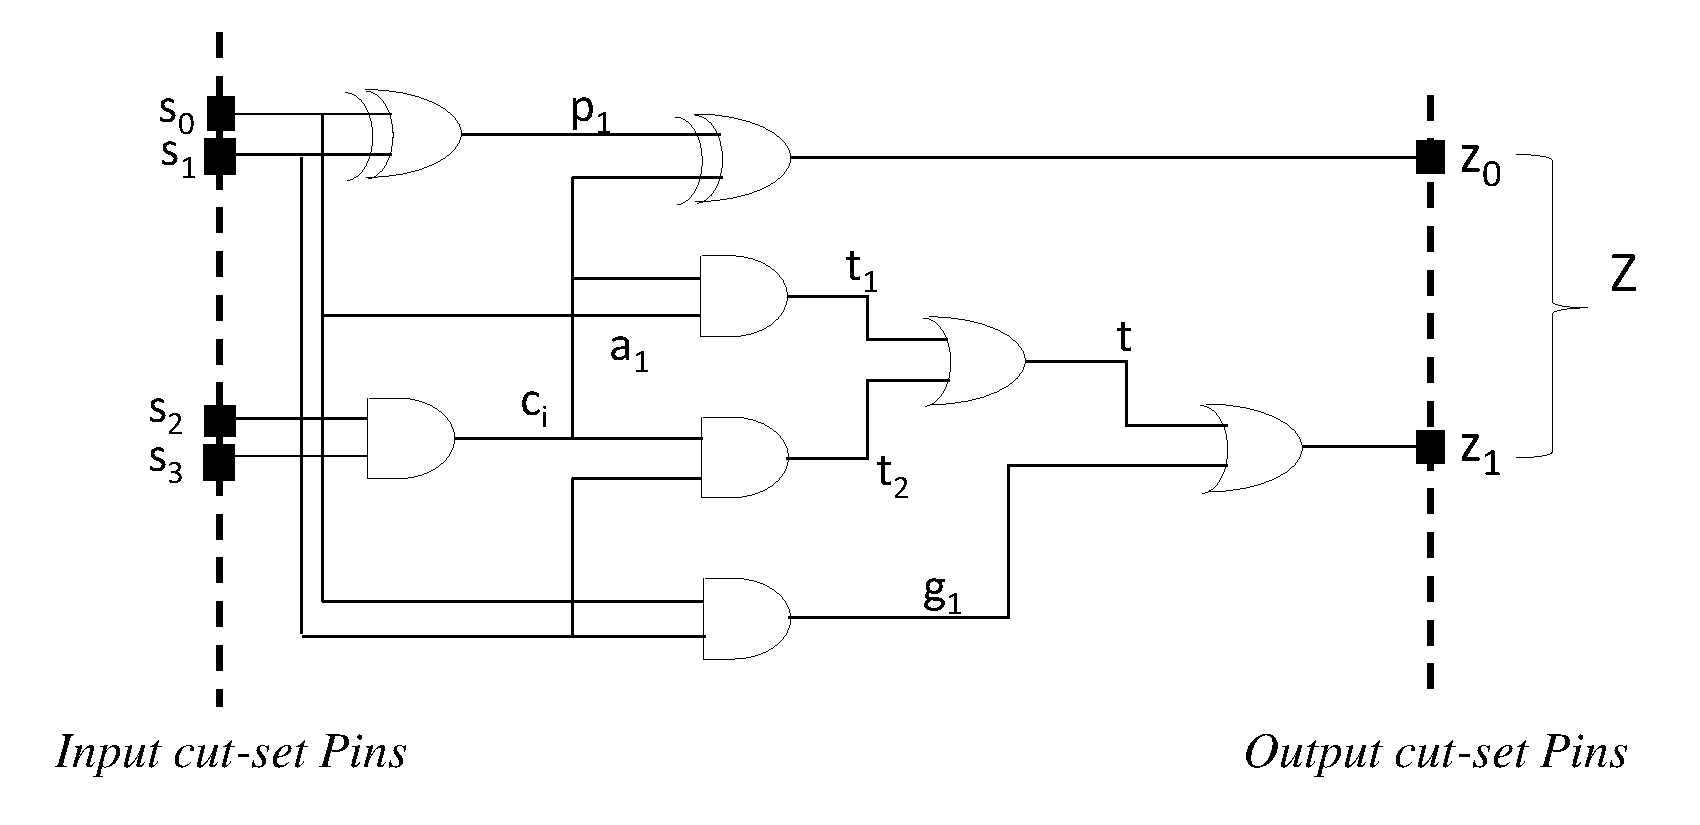
\includegraphics[scale=0.2]{tobemapped.png}
	\end{center}
	\caption{An example gate-level netlist to be mapped}
	\label{fig:tobemapped}
\end{figure}

Fig.\ref{fig:tobemapped} shows an example circuit partition with $a1,b1,a0,b0$ as inputs and
$Z = \{z0,z1\}$ as outputs. If we use elements from Galois field $F_{2^2}$ to represent word $Z$,
we have $Z = z_0 + \alpha\cdot z_1$.

The abstraction also uses the property of Gr\"obner basis. If we arrange a term ordering as
$$Other\ circuit\ variables > output\ word\ Z > all\ bit\ level\ inputs$$
and include all gates information, word level variable definition and vanishing polynomials,
the reduced Gr\"obner basis will have a polynomial (generator) in the form of $Z + f(a1,b1,a0,b0)$,
this is an application of "elimination using GB", where we eliminate all variables except output
word variable $Z$ and inputs $a1,a0,b1,b0$.

In this example:

\begin{itemize}
\item Term ordering: $z0,z1,t,g1,p1,ci,t1,t2,Z,a0,b0,a1,b1$
\item Gate description (from table \ref{table:booltogalois_op}): $z0+t+g1+t\cdot g1, t+t1+t2+t1\cdot t2, g1+a1\cdot b1,
			t1+a1\cdot ci, t2+b1\cdot ci, ci+a0\cdot b0, z1+p1+ci, p1+a1+b1$
\item Word definition: $Z+z0+z1\cdot \alpha$
\item Vanishing polynomials $(J_0)$: $z0^2+z0, z1^2+z1, t^2+t, g1^2+g1, t1^2+t1, t2^2+t2, p1^2+p1, ci^2+ci,
			a0^2+a0, b0^2+b0, a1^2+a1, b1^2+b1, Z^4+Z$(note Z is 2-bit word)
\end{itemize}

The result is one polynomial in Gr\"obner basis with leading term $Z$:
$$Z+a0\cdot b0\cdot a1+a0\cdot b0\cdot b1+\alpha\cdot a0\cdot b0+a1\cdot b1+\alpha\cdot a1+\alpha\cdot b1$$

\begin{table}
\centering
\begin{tabular}{|c|c|} \hline
Boolean operator & operation in $\mathbb{F}_{2}$\\ \hline
$\overline{a}$ & $1 + a$\\ \hline
$a\ and\ b$ & $ab$\\ \hline
$a\ or\ b$ & $a + b + ab$\\ \hline
$a \oplus b$ & $a + b$\\
\hline\end{tabular}
\caption{Some Boolean operators and corresponding operations in $\mathbb{F}_{2}$}
\label{table:booltogalois_op}
\end{table}

\subsection{Templates on Boundary Information}
\begin{figure}[hbt]
	\begin{center}
	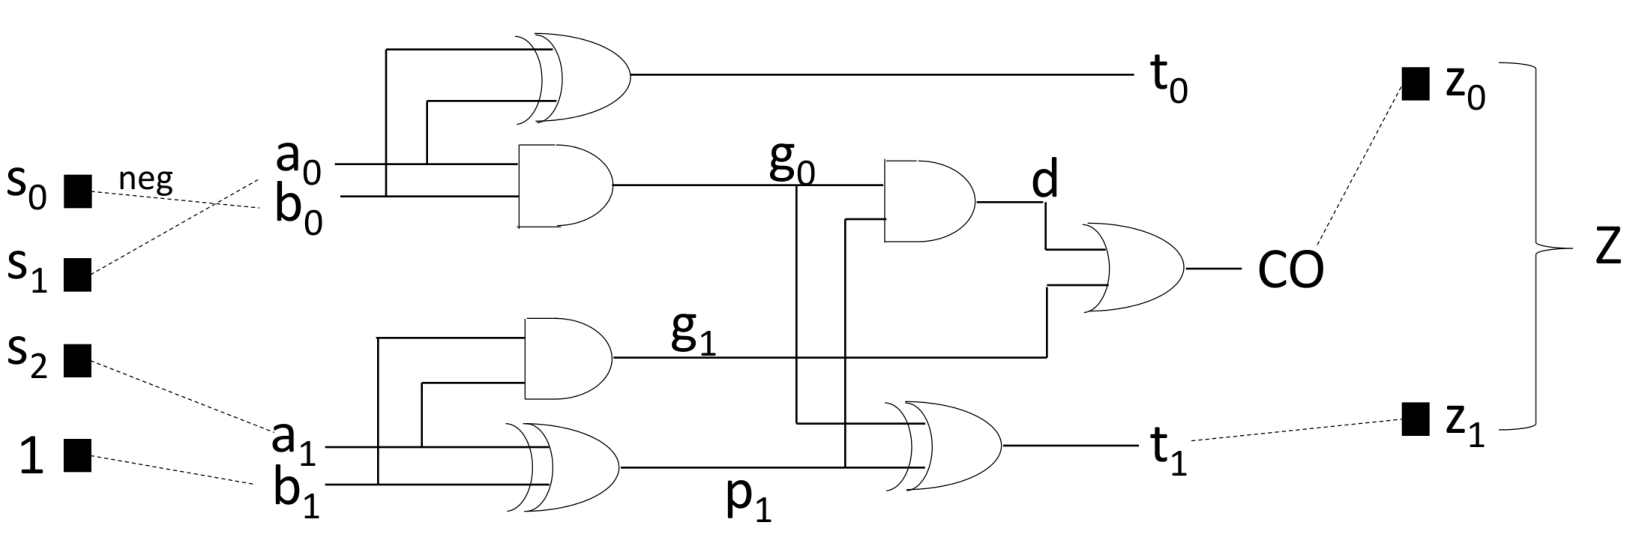
\includegraphics[scale=0.2]{template.png}
	\end{center}
	\caption{Standard 2-bit adder with input/output mapping}
	\label{fig:template}
\end{figure}

Fig.\ref{fig:template} shows a 2-bit standard cell. It has 3 outputs mapping to 2 output pins,
and 4 inputs mapped to 3 input pins (the rest pin is mapped to fixed 0/1 signal). Dashed connection
lines show one possible mapping, to find out this kind of feasible mapping, we need to simulate
all possible mappings, where the concept "template" can be used.\vspace{5mm}

{\bf Output template}: $z0+ct0_{z0}\cdot t0+ct1_{z0}\cdot t1+c0_{CO}\cdot CO+cn0$

When $cn0 = 0$, any one of $ct0_{z0},ct1_{z0},c0_{CO}$ could be 1 means mapping to corresponding output
pin. If $cn0 = 1$, mapping to negation of corresponding output pin.

{\bf Input template}: $a0+pa0+c0_{A0}\cdot s0+c1_{A0}\cdot s1+c2_{A0}\cdot s2$

When $pa0 = 0$ and any one of $c0_{A0},c1_{A0},c2_{A0}$ equal to 1 means mapping to corresponding input
pin; if all $c0_{A0},c1_{A0},c2_{A0}$ equal to 0 then means mapping to fixed signal "0" (when $pa0 = 1$ then
mapping to fixed signal "1").

\subsection{Fast GB computing}
We compose an ideal with polynomials from all gates information, input/output templates and word definition,
then compute a GB of this ideal. However, computing GB using algorithms like Buchberger's algorithm is
less efficient. For example, the "slimgb" function in Singular tool cannot even compute a GB for ideal
from Fig.\ref{fig:template}. So finding a fast GB computing method is necessary.

Analyzing Buchberger's algorithm, we find the reason that GB compute takes long time is the size of ideal
will explode when there exists many pairs of polynomial can compute a Spoly. If we arrange the term ordering
carefully to minimize the number of Spoly, then GB computation will be easy.

We find such term ordering can satisfying our requirement:
\begin{align}
&Reverse\ topological\ order\ of\ circuit\ variables > \nonumber\\
& output\ word\ variable > output\ templates\ variables>\nonumber\\
& fixed\ 0/1\ templates\ variables > input\ templates\ var\nonumber\\
& > input pins \nonumber
\end{align}

Under this term ordering, all polynomials' leading term are relatively prime (so Spoly equal to 0)
except only 1 pair of polynomials. So the work load is just compute a Spoly for this pair,
then reduce the Spoly with whole ideal. After adding the remainder to the ideal, it becomes
a Gr\"obner basis.

\subsection{Our Tool Flow}
First, choose a set of independent wires as input pins;

Second, push forward input signal for a certain number of gates (depth), choose a cut set
which fully dependent on these inputs as output pins;

Third, abstract a description polynomial using GB abstraction method;

Fourth, reduce (do multi-division) the description polynomial with the GB we computed with macro block 
and templates, get a remainder polynomial;

Last but not least, abstract all coefficients from the remainder polynomial, set up a system of equations,'
find a solution to this system, then the solution is a feasible mapping; no solution means cannot make a
feasible mapping.

\section{Problems to address}
The final system of equations is not linear, so a 0/1 programming technique cannot be used. However,
an exhaustive enumerating is still practicable:
If we map a marco block with $j$ inputs and $n$ outputs into circuit partition with $i$ inputs
and $m$ outputs, number of total possible assignments is
$$2^{j-i}A_j^iA_n^m$$
when considering mapping to negative signals, it increases to 
$$2^{m+j}A_j^iA_n^m$$

For example, when mapping 3 inputs 2 outputs partition to a 2-bit adder:

Total possible assignments: 9216

Full search space: $2^{24} = 16.8M$

So it only takes $0.05\%$ time to scan all possibilities using our approach.

When the macro block is larger as 4-bit adder, number of total possible assignment is $2^{27}$,
still a number we can accept.
%%%%%%%%%%%%%%%%%%%% The bibliography %%%%%%%%%%%%%%%%%%%%%%%%%%%%
%\begin{thebibliography}{1}
%\bibitem{ref1}
%\end{thebibliography}
\end{document}


%%%%%%%%%%%%%%%%%%%%%%%%%%%  End of IEEEsample.tex  %%%%%%%%%%%%%%%%%%%%%%%%%%%